\chapter{Implementation}
This section deals with the realization of technical specification , design, software component and standard algorithm. It includes methods which are implementations of those methods specified by the interface.

\section{Tools and Technologies}

\subsection{NodeJS}

Node.js is an open-source, cross-platform JavaScript run-time environment that executes JavaScript code server-side. Historically, JavaScript was used primarily for client-side scripting, in which scripts written in JavaScript are embedded in a webpage's HTML and run client-side by a JavaScript engine in the user's web browser. Node.js lets developers use JavaScript to write command line tools and for server-side scripting—running scripts server-side to produce dynamic web page content before the page is sent to the user's web browser. Consequently, Node.js represents a "JavaScript everywhere" paradigm, unifying web application development around a single programming language, rather than different languages for server side and client side scripts. 

NodeJS has been used to write the complete back-end of our mini-project for creating RESTful APIs that are used to integrate back-end with the front.  

\subsection{MongoDB}

The database used for this project is MongoDB which is a free and open-source cross-platform document-oriented database program. MongoDB uses JSON-like documents with schemas and is classified as a NOSQL database. It is published under a combination of the GNU Affero General Public License and the Apache License.

This is a NOSQL database so our need is easily fulfilled using this database as it stores data in document format using key-value pairs and js also works on json objects, thus simplifying the task of retrieving and manipulating the data.

\subsection{ReactJS}
ReactJS is a javascript library which is used for creating user interfaces. React makes it easy to maintain the front-end. As our project is a modular based project where all the features have been implemented as different modules, react, which uses a component based approach to developing user interfaces, can go hand-in-hand with the back-end. Due to this very nature of react, we can easily scale it in future too. Moreover, react is very lightweight thus takes less loading time. Hence, it’s really convenient for designing our project’s user Interface.


\section{Coding Standards Followed}

\subsection{Proper Indentation / Structure}
The entire code is properly indented with uniform spaces and also leaving spaces between operands and operators. All the modules to be imported are imported at the top of the files, thus making the code clearer and easy to understand.

\subsection{Naming Convention}
The variables are given meaningful names and naming is performed using camel case variable naming convention. This makes the code neater and the code becomes more meaningful and easy to understand.

\subsection{Avoiding Callback Hell}
All the functions written inside the controller are designed using the async-await approach using promises, thus avoiding callbacks almost completely. This makes the code much more linear avoiding the deeply nested structure which results due to using callbacks, called the callback hell. We have successfully avoided that problem by writing all the functions using async-await approach.

\subsection{Modular Approach}
Each feature has been implemented as a completely independent function which is exported by the controller module. The functioning of each and every one of these functions does not depend or effect the functioning of other functions. This makes the addition and removal of new features easy. Also, debugging has been made easy due to this approach.

\subsection{Proper Folder Structure/Naming}
A standard folder structure has been followed in the project, keeping all the related files in different folders. The files containing the core functions are kept inside controller folder, all the api end-point containing files are kept inside routes folder, all the database schema models are kept inside models folder.

\subsection{Model View Controller Model}
Model–View–Controller (usually known as MVC) is an architectural pattern commonly used for developing user interfaces that divides an application into three interconnected parts. This is done to separate internal representations of information from the ways information is presented to and accepted from the user. The MVC design pattern decouples these major components allowing for efficient code reuse and parallel development.

\subsection{Documentation}
All the API end-points have been properly documented to make the integration easier and clear. The documentation contains the type of request to be sent to a specified route along with all the required input and the expected output along with all the constraints and error possibilities.

\pagebreak

\section{Execution Results and Discussions}

This section shows the execution results after integration and deployment. We shall be looking at some of the screenshots of the user interface which will outline the functioning of our app.


\subsubsection{}

\begin{center}
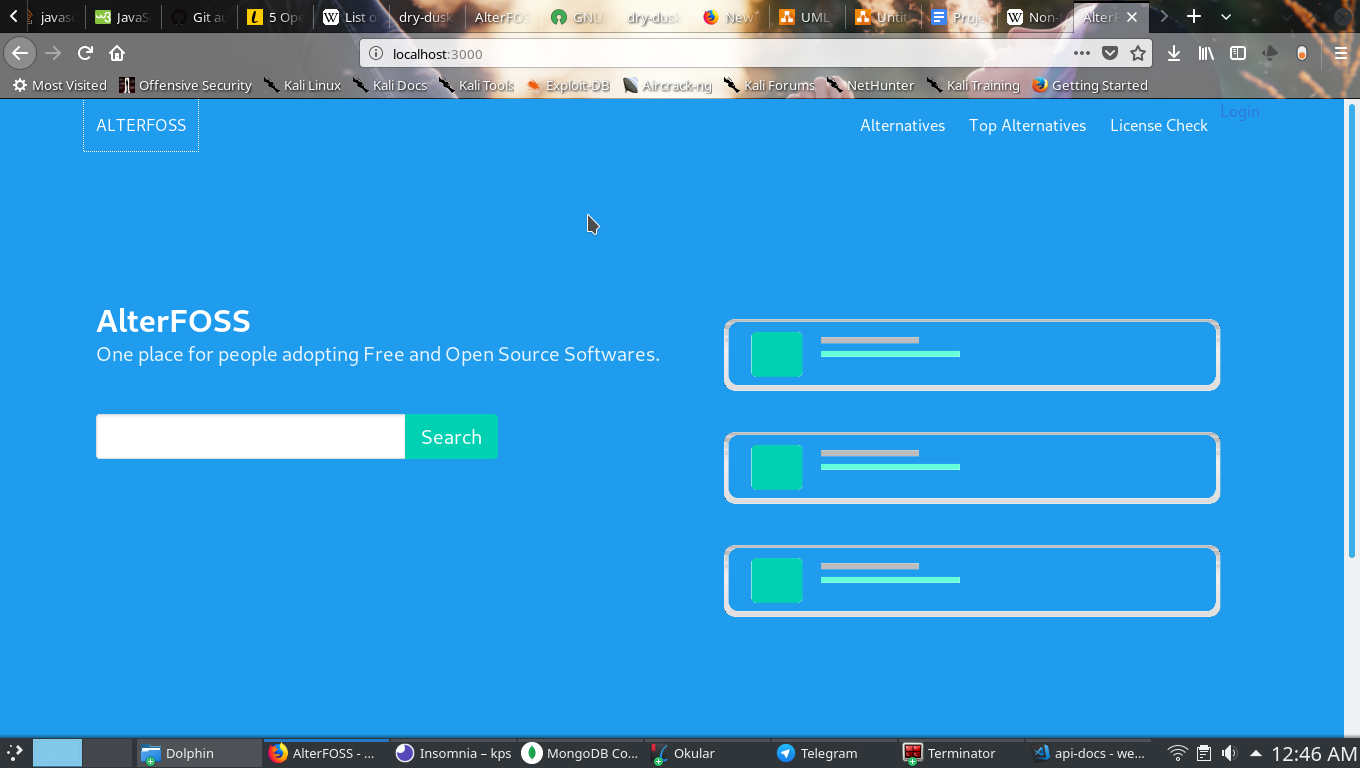
\includegraphics[scale=0.45]{images/4-1.png}
\captionof{figure}{Home Page}
\end{center}


The figure shown above is the home page of our web Application. The various links can be seen above such as alternatives to get alternatives for proprietary softwares, top alternatives which is used to list out the top 10 alternatives based on upvotes. License check is used to check the license information of alternatives. The search bar shown here is used to search proprietary softwares based on the text the user passes via this text box.

The below figure (fig. 4.2) shows proprietary search results for search query “windows”. This search is performed by treating the input text as regular expression. The information displayed is the name of the proprietary software along with the description of the software in the order in which it was found.

\subsubsection{}
\begin{center}
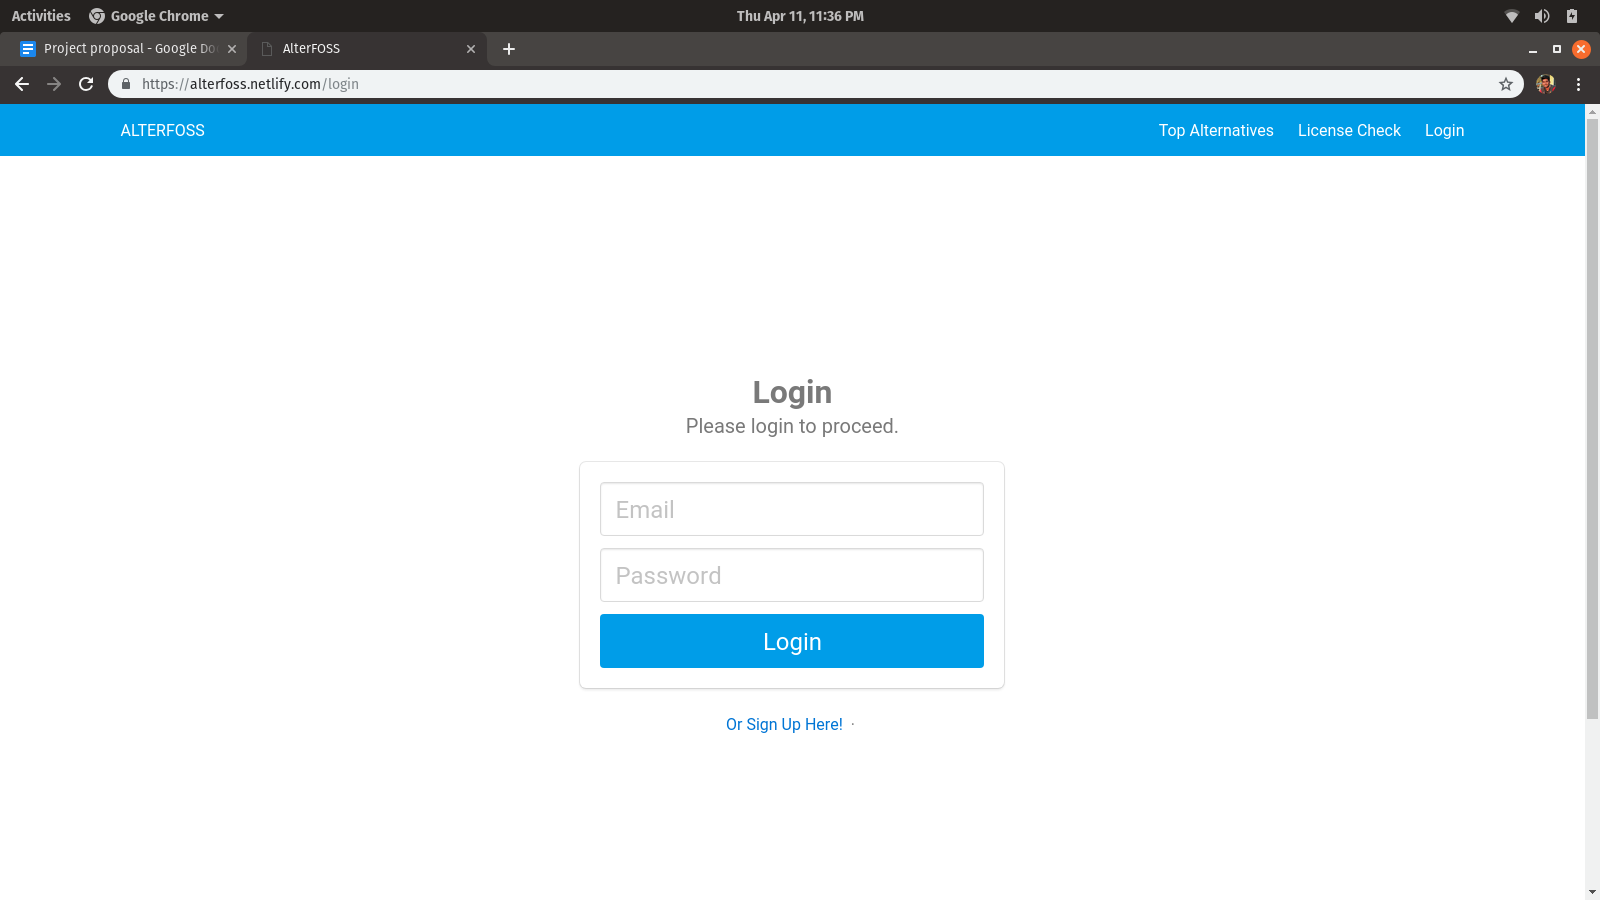
\includegraphics[scale=0.29]{images/login.png}
\captionof{figure}{Home Page}
\end{center}


\begin{center}
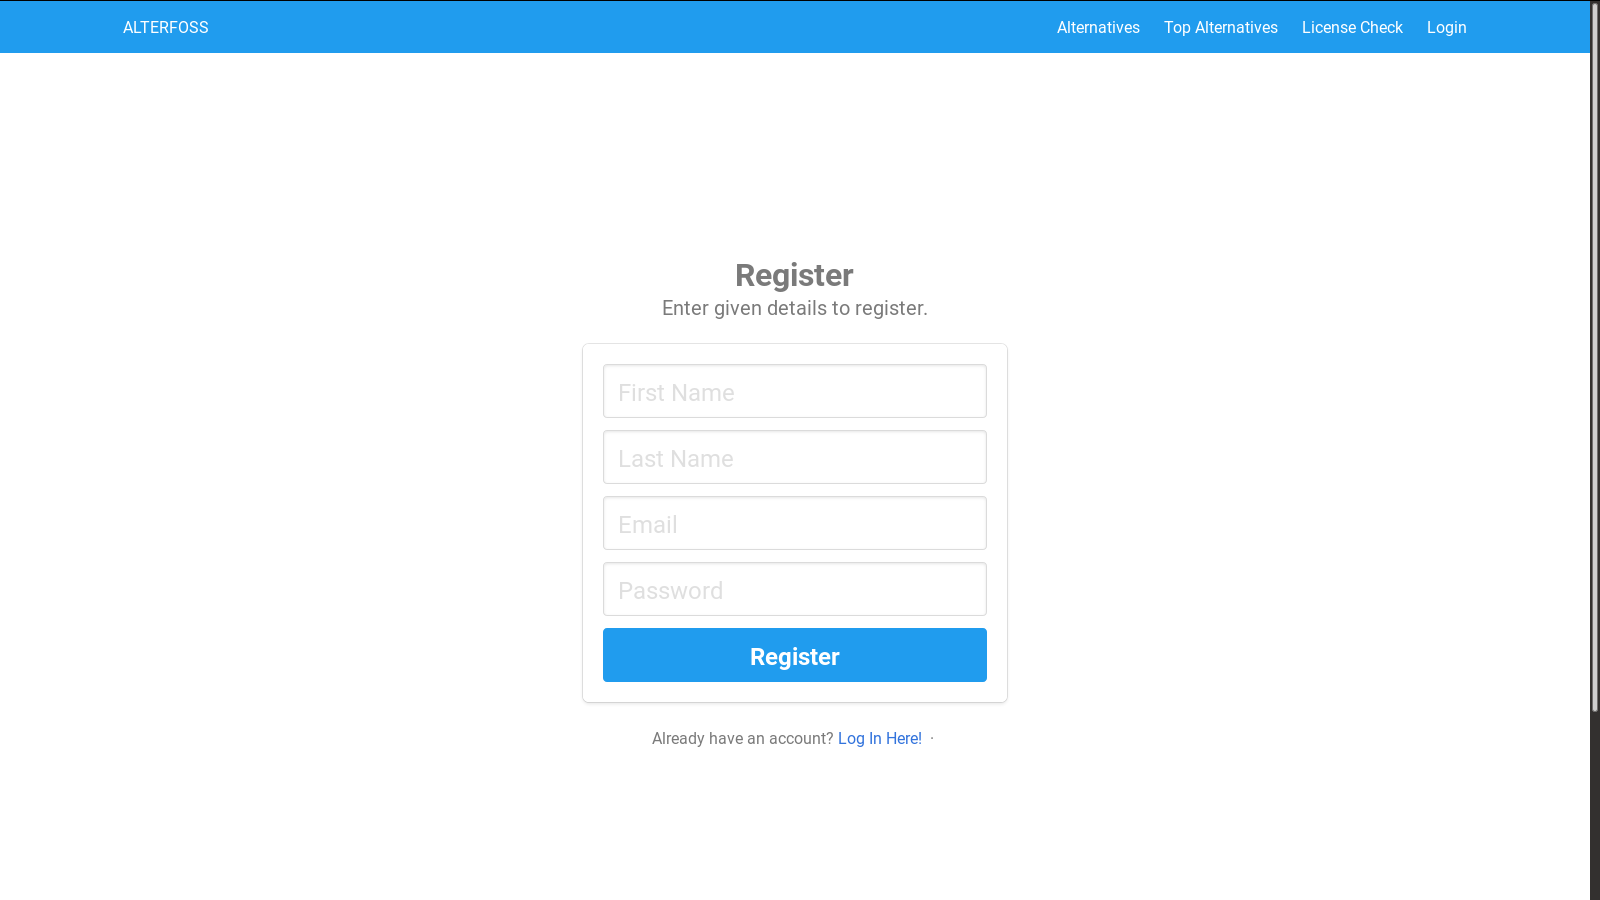
\includegraphics[scale=0.29]{images/register.png}
\captionof{figure}{Home Page}
\end{center}

Figures 4.2 and 4.3 show the authentication interfaces of the application.


\subsubsection{}

\begin{center}
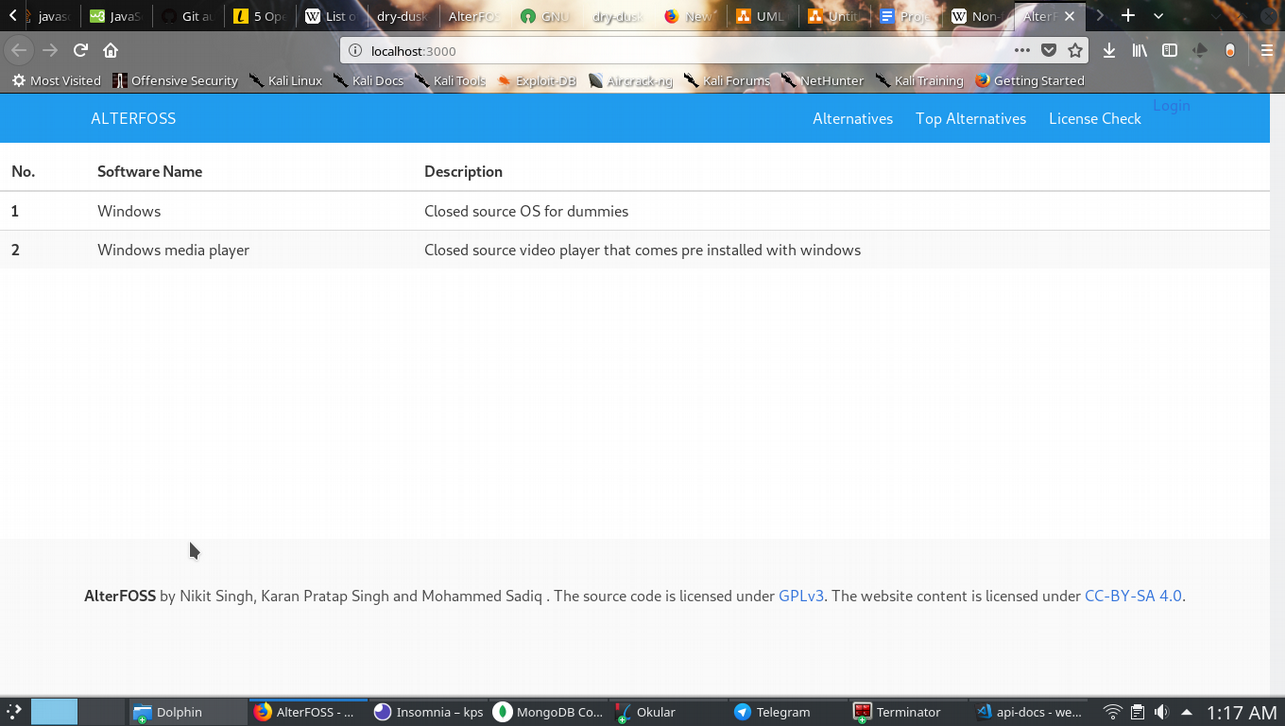
\includegraphics[scale=0.45]{images/4-2.png} 
\captionof{figure}{Proprietary Search Results}
\end{center}

In fig. 4.4, we had searched for 'windows media player' and those were the replies we got.

\subsubsection{}

\begin{center}
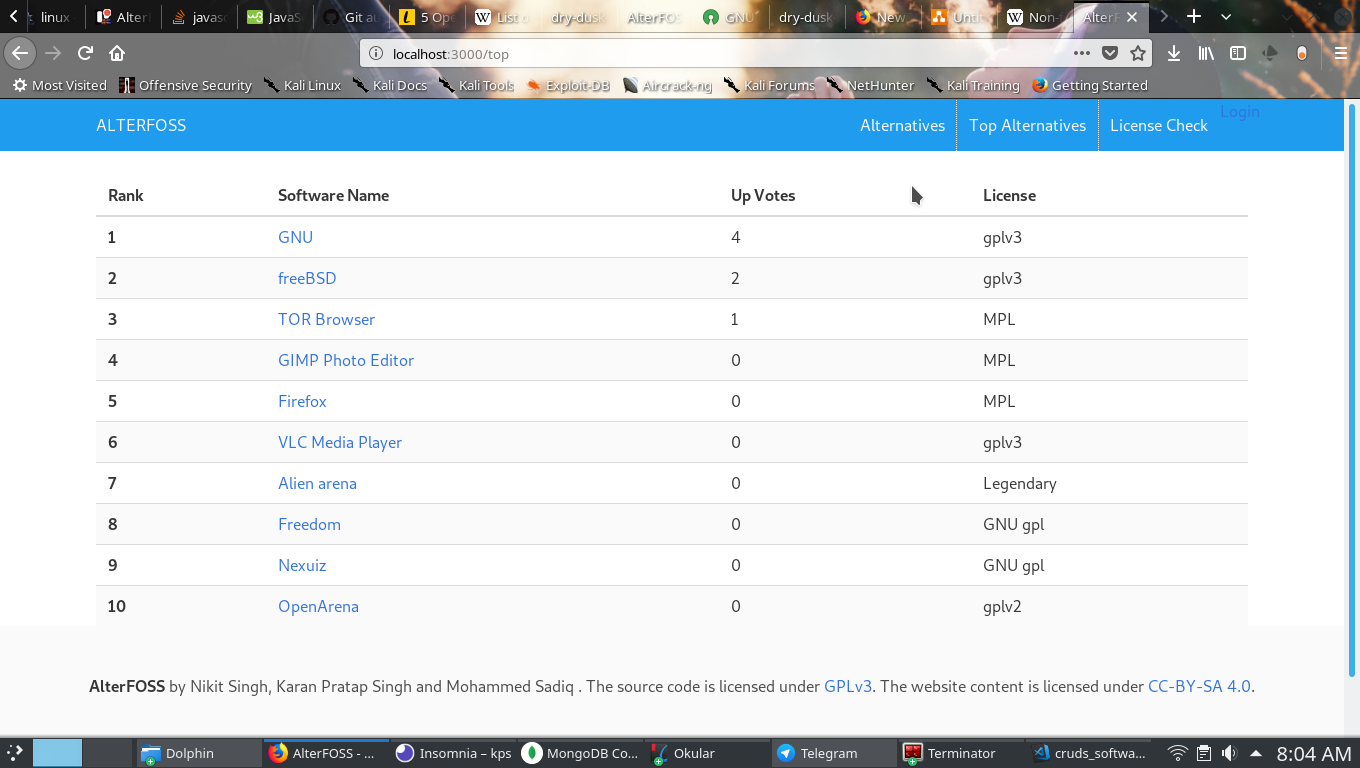
\includegraphics[scale=0.43]{images/4-3.png}
\captionof{figure}{Top 10 alternatives}
\end{center}

As shown in fig. 4.5, the top 10 alternatives list can be viewed by the user by clicking on top alternatives option on the top right of the web page. It will display the list of top 10 alternatives along with their upvotes and license. This list is sorted, as discussed previously, based on the number of upvotes of the software. The api fetches the top 10 alternatives from the database, sorts them and sends them to the front end for display.


\subsubsection{}

\begin{center}
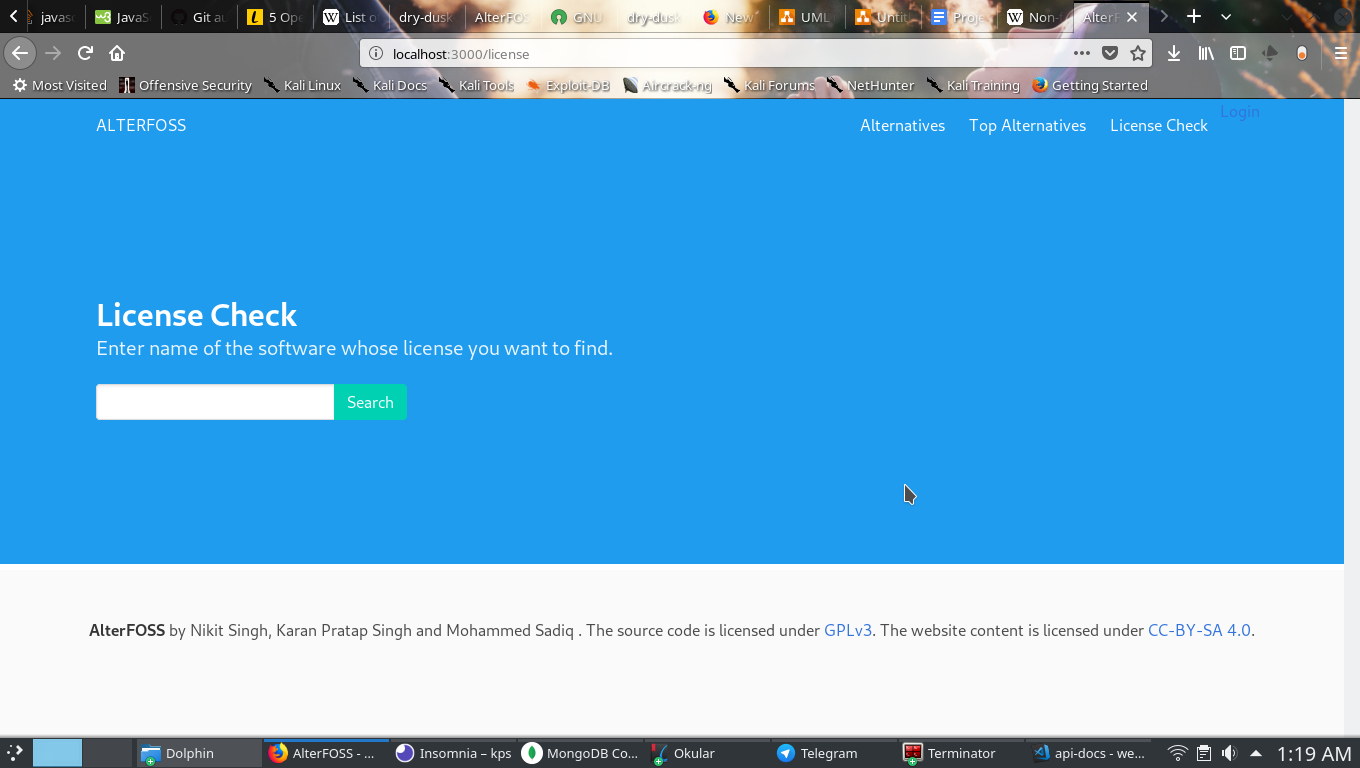
\includegraphics[scale=0.44]{images/4-4.png}
\captionof{figure}{License Checker}
\end{center}

The above depicted is the license checker module implemented in our mini project. The user can provide search text in the given text box to search alternative softwares. The result will be the name of the alternatives matching this search string along with their license information. Thus, the user can get the license information of any proprietary software he desires using this module.

The result of this query is as shown in the following figure (fig. 4.5), which shows the search result for the search query ‘tor’. Since the items are matched with the search pattern using the regExp approach with case insensitive flag set, thus this search leads to displaying both TOR browser and GIMP photo editor.

\begin{center}
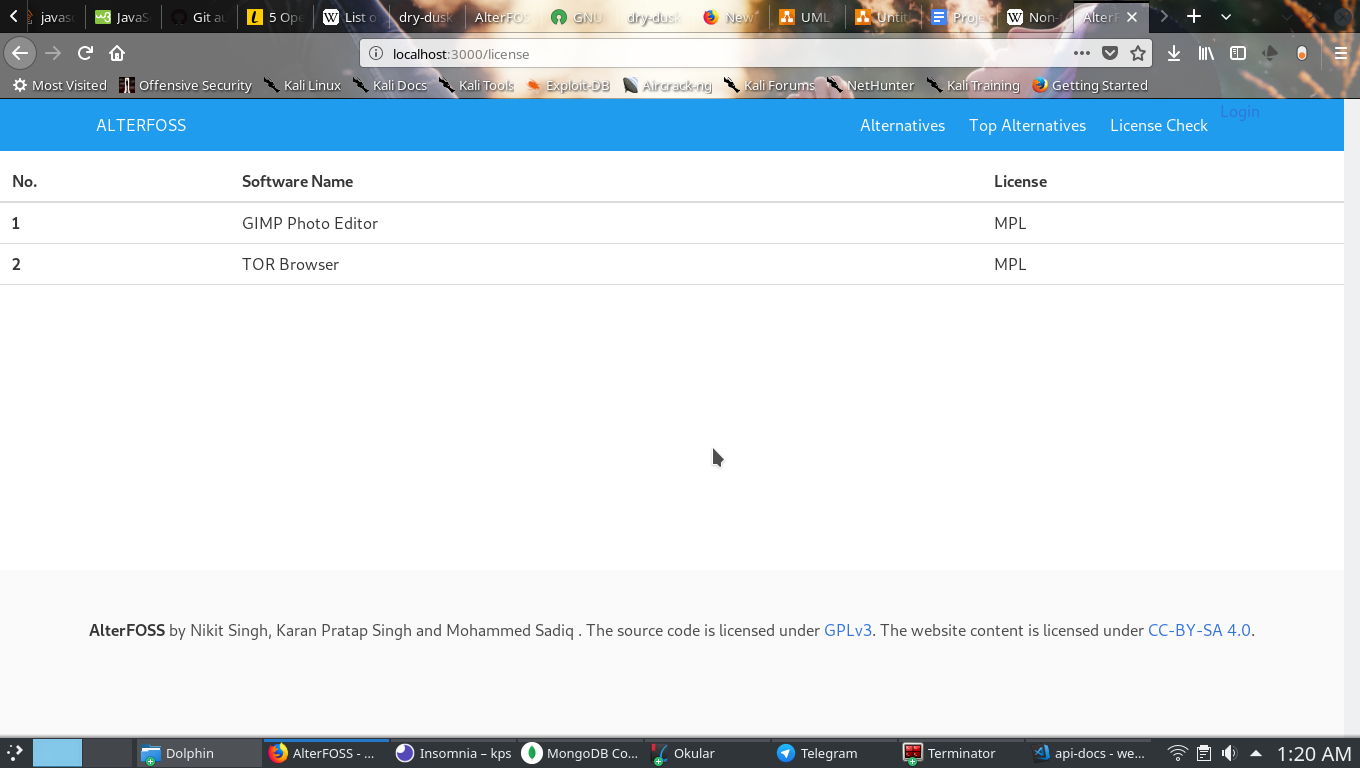
\includegraphics[scale=0.45]{images/4-5.png}
\captionof{figure}{License Checker Output}
\end{center}

\begin{center}
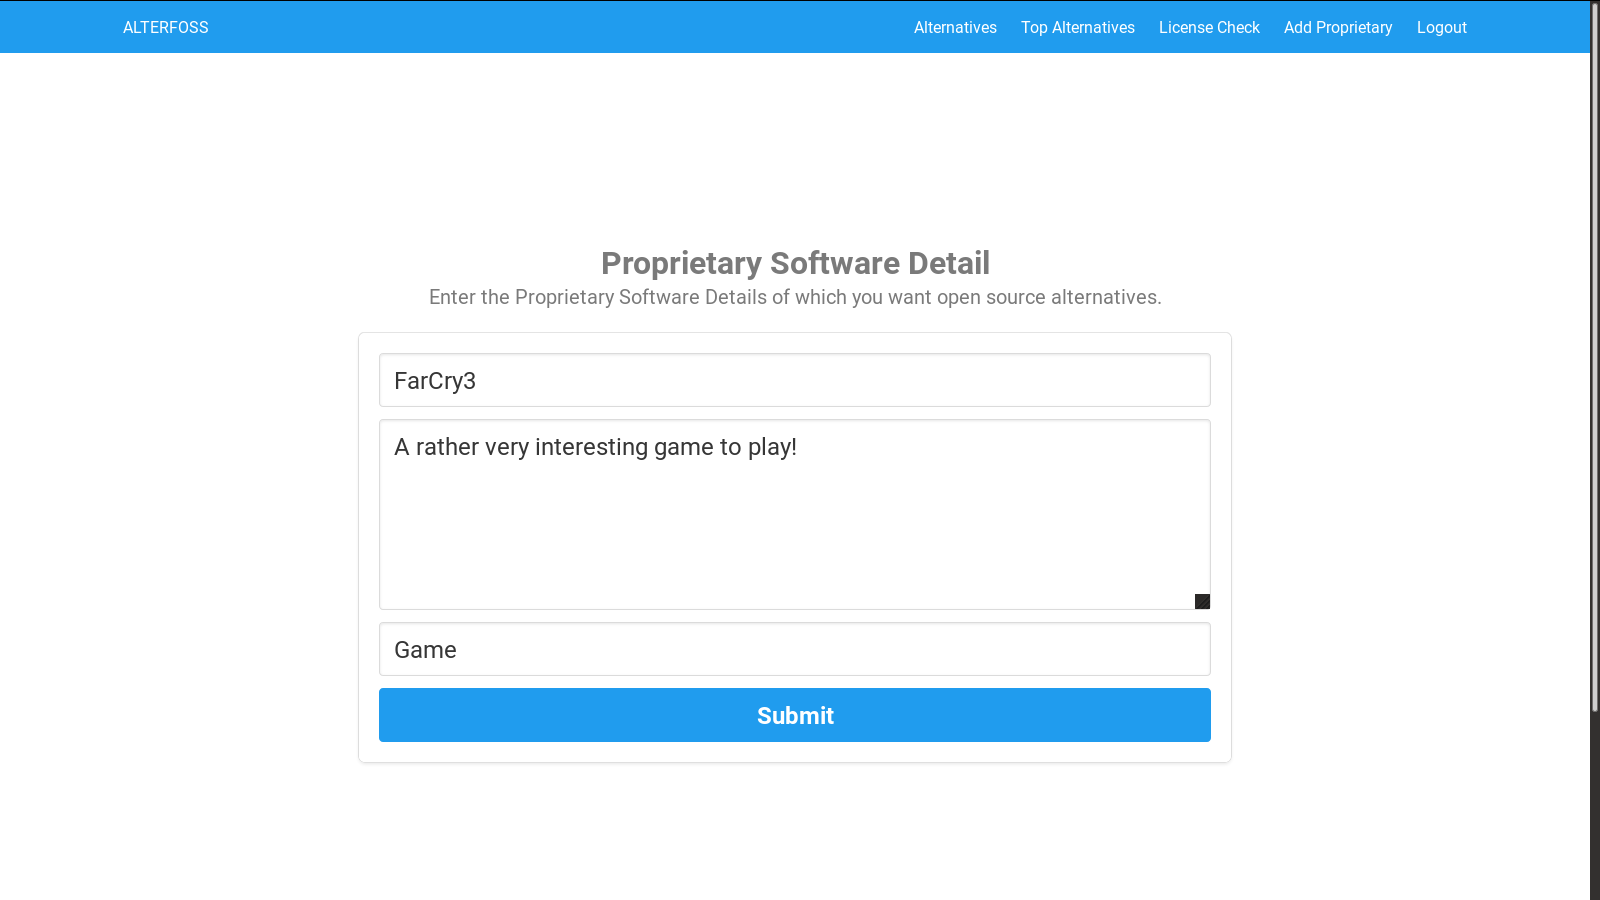
\includegraphics[scale=0.285]{images/4-6.png}
\captionof{figure}{Adding a new proprietary software}
\end{center}

As can be seen from the above figure, the user will have to provide the details of the software such as name, short description and tags via a form in order to request for this proprietary software's alternatives. The requested-by field will be set to anonymous automatically if the user is not logged in. Otherwise, the username will be fetched from the current session and will be assigned to the requested-by field. A json object will be created using these details fetched from the user and this object is sent via the req.body property of the request. In response, the back-end will return the complete object written onto the database along with the \_id and \_v fields(though these can't be seen in the figure explicitly).


\begin{center}
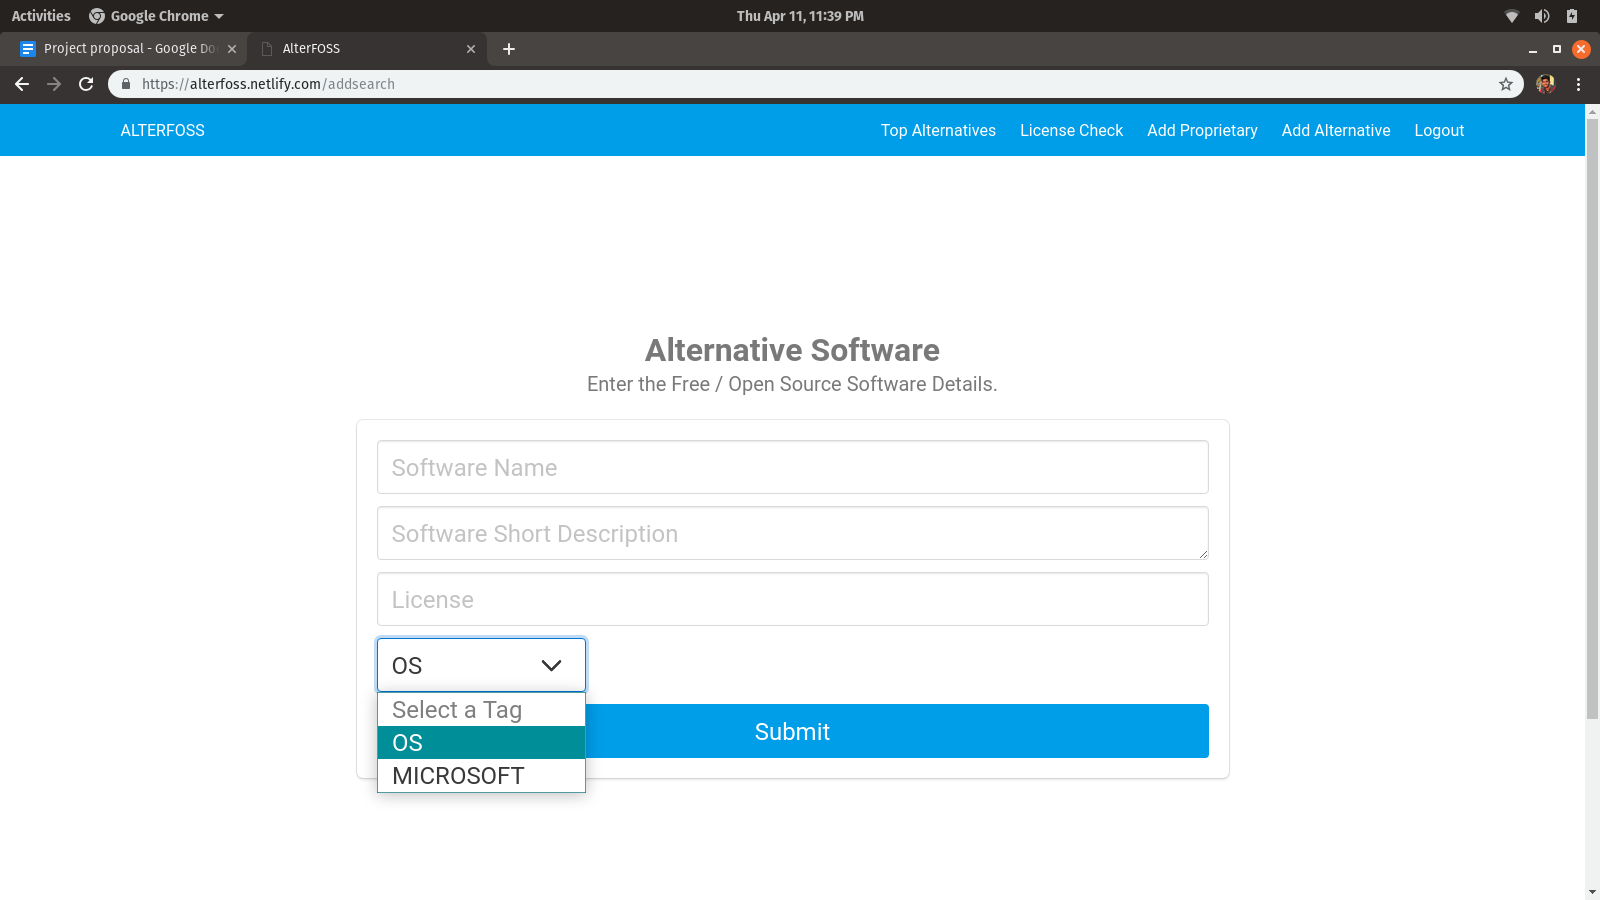
\includegraphics[scale=0.285]{images/4-7.png}
\captionof{figure}{Creating a new alternative}
\end{center}


Once the proprietary software is requested by someone as shown previously, the other community members will have the option to suggest alternatives for this proprietary software. This feature is also quite similar to that of the addition of proprietary software. The user needs to specify the name, license, short description and a handle for the alternative to be added. A json object is created using these properties and setting their values to those specified by the user via the front-end form. Here also, the suggested by field is set to the username from the current session, in case the user is logged in, otherwise the default value ‘anonymous’ is used.
Both of these features to add an alternative and to create a proprietary software requires a ‘POST’ request to be sent to the server. These softwares are then stored inside the database and can be viewed by other users later. This way the platform will keep growing and the community will steer it.


\subsubsection{}


\begin{center}
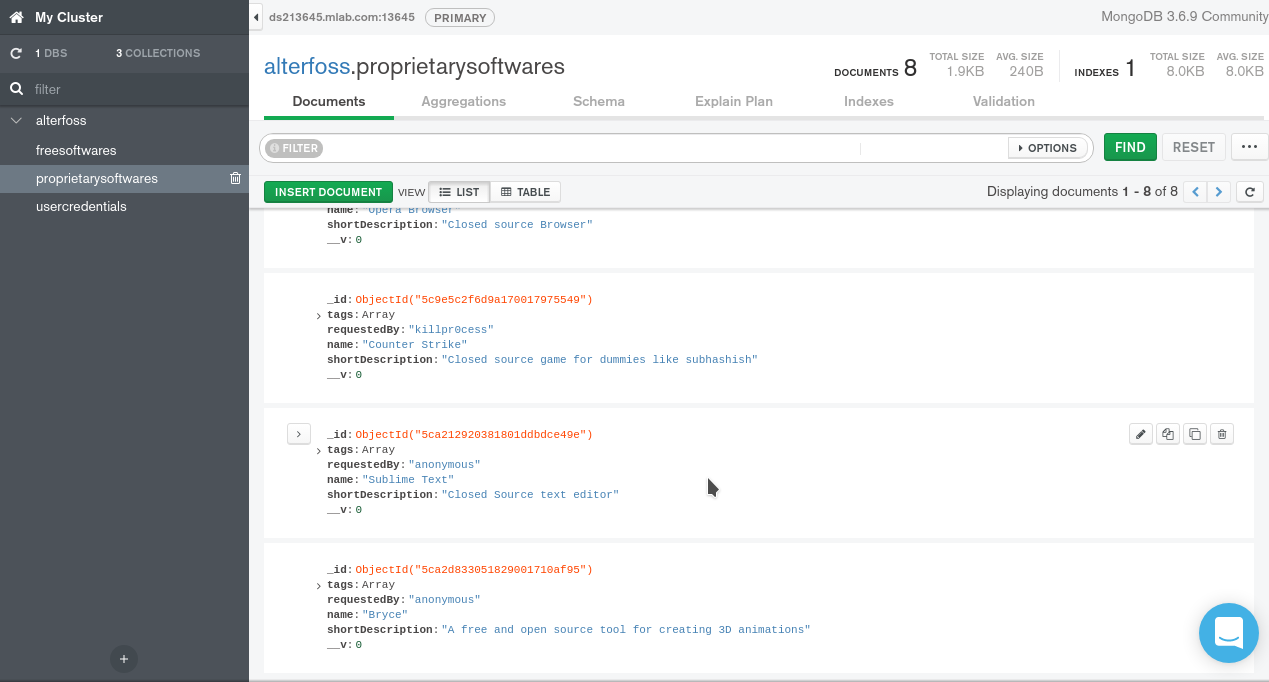
\includegraphics[scale=0.47]{images/4-8.png}
\captionof{figure}{proprietarySoftware collections}
\end{center}



\begin{center}
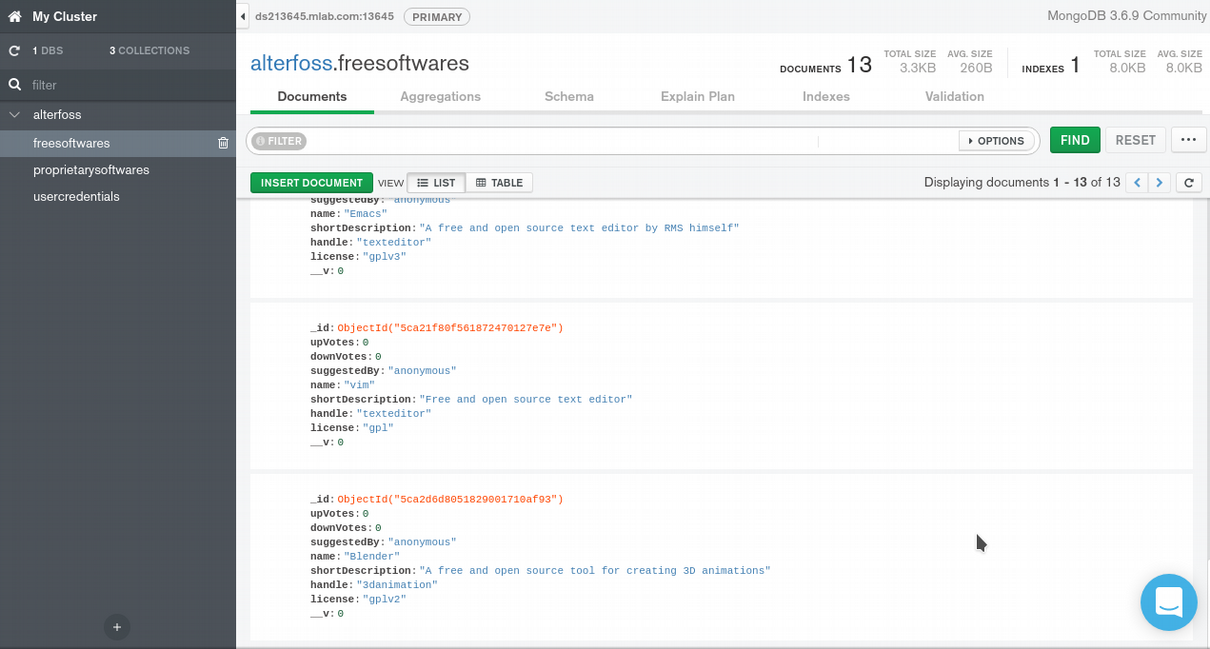
\includegraphics[scale=0.5]{images/4-9.png}
\captionof{figure}{freeSoftwares collections}
\end{center}

The above screenshots (fig. 4.10 and fig. 4.11) show a glimpse of the database after addition of these softwares.

























